%%%%%%%%%%%%%%%%%%%%%%%%%%%%%%%%%%%%%%%%%
% Masters/Doctoral Thesis 
% LaTeX Template
% Version 1.43 (17/5/14)
%
% This template has been downloaded from:
% http://www.LaTeXTemplates.com
%
% Original authors:
% Steven Gunn 
% http://users.ecs.soton.ac.uk/srg/softwaretools/document/templates/
% and
% Sunil Patel
% http://www.sunilpatel.co.uk/thesis-template/
%
% License:
% CC BY-NC-SA 3.0 (http://creativecommons.org/licenses/by-nc-sa/3.0/)
%
% Note:
% Make sure to edit document variables in the Thesis.cls file
%
%%%%%%%%%%%%%%%%%%%%%%%%%%%%%%%%%%%%%%%%%

%----------------------------------------------------------------------------------------
%	PACKAGES AND OTHER DOCUMENT CONFIGURATIONS
%----------------------------------------------------------------------------------------

\documentclass[11pt, oneside]{Thesis} % The default font size and one-sided printing (no margin offsets)

\graphicspath{{Pictures/}} % Specifies the directory where pictures are stored
\usepackage{wrapfig}
\usepackage{graphicx}
\usepackage{caption}
\usepackage{subcaption}
\usepackage{amsmath}

\usepackage[square, numbers, comma, sort&compress]{natbib} % Use the natbib reference package - read up on this to edit the reference style; if you want text (e.g. Smith et al., 2012) for the in-text references (instead of numbers), remove 'numbers' 
\hypersetup{urlcolor=blue, colorlinks=true} % Colors hyperlinks in blue - change to black if annoying
\title{\ttitle} % Defines the thesis title - don't touch this

\begin{document}

\frontmatter % Use roman page numbering style (i, ii, iii, iv...) for the pre-content pages

\setstretch{1.1} % Line spacing of 1.3

% Define the page headers using the FancyHdr package and set up for one-sided printing
\fancyhead{} % Clears all page headers and footers
\rhead{\thepage} % Sets the right side header to show the page number
\lhead{} % Clears the left side page header

\pagestyle{fancy} % Finally, use the "fancy" page style to implement the FancyHdr headers

\newcommand{\HRule}{\rule{\linewidth}{0.5mm}} % New command to make the lines in the title page

% PDF meta-data
\hypersetup{pdftitle={\ttitle}}
\hypersetup{pdfsubject=\subjectname}
\hypersetup{pdfauthor=\authornames}
\hypersetup{pdfkeywords=\keywordnames}

%----------------------------------------------------------------------------------------
%	TITLE PAGE
%----------------------------------------------------------------------------------------

\begin{titlepage}
\begin{center}

\textsc{\LARGE Imperial College London}\\[1.5cm] % University name
\textsc{\Large Interim Report}\\[0.5cm] % Thesis type

\HRule \\[0.4cm] % Horizontal line
{\huge \bfseries Turning Music Into Game}\\[0.4cm] % Thesis title
\HRule \\[1.5cm] % Horizontal line
 
\begin{minipage}{0.4\textwidth}
\begin{flushleft} \large
\emph{Author:}\\
\href{pak11@doc.ic.ac.uk}{Paulina Koch} % Author name - remove the \href bracket to remove the link
\end{flushleft}
\end{minipage}
\begin{minipage}{0.4\textwidth}
\begin{flushright} \large
\emph{Supervisor:} \\
Dr. Iain Phillips \\ \vspace{20pt}
\emph{2nd Marker:} \\
Dr. Robert Chatley
\end{flushright}
\end{minipage}\\[3cm]
 
 
{\large \today}\\[4cm] % Date
%\includegraphics{Logo} % University/department logo - uncomment to place it
 
\vfill
\end{center}

\end{titlepage}


%----------------------------------------------------------------------------------------
%	THESIS CONTENT - CHAPTERS
%----------------------------------------------------------------------------------------

\tableofcontents


\mainmatter % Begin numeric (1,2,3...) page numbering

\pagestyle{fancy} % Return the page headers back to the "fancy" style

% Include the chapters of the thesis as separate files from the Chapters folder
% Uncomment the lines as you write the chapters

% Introduction

\chapter{Introduction} % Main chapter title

\label{Chapter3} % For referencing the chapter elsewhere, use \ref{Chapter1} 

\lhead{Chapter 3. \emph{Introduction}} % This is for the header on each page - perhaps a shortened title

%----------------------------------------------------------------------------------------

\begin{quotation}
Music and games share a fundamental property: both are playable, offering their listeners and operators an expressive experience with the framework of melody and rhythm \cite{introquote}.
\end{quotation} 

As the quote suggests, both games and music have one thing in common — the act of playing. Just as player’s character might die in an attempt to complete a level, causing him to lose the game, the pianist can fail at the attempt of performing a musical piece. 

Perhaps this analogy inspired programmers to develop a new genre of games - music games, where players interact with music. Possibly the most commonly known franchises in this genre are Guitar Hero, Rock Band and Dance Dance Revolution. In this type of games user has to follow the indicators on the screen telling him which buttons to hit. 

The concept of a music game stormed the industry in 2005, after Guitar Hero was released. The project was soon announced the fastest video game franchise to reach \$1 billion in retail sales in the history of the business, with Guitar Hero III being the first single game to reach \$1 billion \cite{GHSales}.

However, a limited amount of songs transcribed and adjusted to the gameplay soon caused the popularity of such music video games to decline. Some brave fans of the franchises took it upon themselves to transcribe songs to create new levels. The producers, seeing the tendency, started releasing the in-app purchases to enable the players to extend their library and thus, keep the users. 

There exist some tools that allow users to manually add new songs to those games, but they are hack-arounds, created by frustrated users, and not real solutions. Moreover, due to the time consuming and difficult nature of the process, most players usually limit themselves to preprocessed songs provided by the game producers, not really taking advantage of the full capabilities of the games. 

This project aims to change the way users look at the music rhythm games. We create a game which allows them to upload any music track they would like and automatically generate a Guitar Hero-like song corresponding to it. 

This is achieved by use of a melody extraction from polyphonic music signals algorithm using pitch contour characterisation. The algorithm consists of four parts - sinusoid extraction, salience function, pitch contour creation and melody selection. In this approach, pitch contours - time continuous sequences of pitch candidates, are grouped using auditory streaming cues. To filter them, a set of contour characteristics, which help distinguish between melodic and non-melodic contours, is defined. This leads to the development of new voicing detection, octave error minimisation and melody selection techniques \cite{salamon}. Once the pitch of the main melody is estimated, we perform further post-processing to remove the unlikely outliers, as well as adjust the difficulty of the song generated according to our needs.

In this project, we also design and develop an algorithm for mapping the estimated pitches of the main melody to a series of buttons on the screen to create an interesting and challenging game for a user, as no literature describing such problem was found so far.

In addition to this, we attempt to develop a mood extraction system to dynamically generate surroundings in the game. Specifically, we treat music emotion recognition as a regression problem to predict the arousal and valence (AV) values of each music sample directly, which then can be used to generate unique surroundings for every song analysed. This continuous view of music emotion makes the proposed music emotion recognition system free of the inherent ambiguity issue. In addition to this, because there is more freedom in describing a song compared to defining and assigning mood classes, the subjectivity issue is alleviated to some extent. \cite{mood}.

The music emotion recognition problem is tackled by designing and training a neural network to predict listeners’ mean valence and arousal ratings associated with musical pieces. Thanks to training on short excerpts, we can then activate the network on parts of the music track uploaded by the user to be able to accurately extract and visualise the mood changes that exist in it.

Moreover, we implement a system to retrieve segments of the music track. This is achieved by identifying the boundaries between parts and labelling them in a way that is clear and understandable to a user. This way we are able to notify the them of their progress in the gameplay, as well as apply more granularity in the mood detection by predicting the emotion on a per segment basis.

This is achieved by generating two self-similarity matrices - one for harmonic pitch class profiles and one for Mel-frequency cepstrum coefficients in a song and decomposing them using Convex Non-Negative Matrix Factorisation and using the results to detect boundaries of a song. The bounds are then used to create a novel algorithm that takes the estimated pitches of the main melody into account for labelling the segments of the song defined by them.

With this project we also show that sophisticated academic music analysis techniques can be combined together and applied to real world problems in an efficient and reliable manner. 

Finally the project aims to be more than just a research study of feasibility. The result of successful completion will be an application of sufficient reliability and quality that it can be released to, and used by, untrained computer users. To our knowledge, it is the only computer game allowing people to generate Guitar Hero-like songs that also generates the surroundings tailored to every music track.


% Background

\chapter{Background} % Main chapter title

\label{Chapter2} % For referencing the chapter elsewhere, use \ref{Chapter2} 

\lhead{Chapter 2. \emph{Background}} % This is for the header on each page - perhaps a shortened title

%----------------------------------------------------------------------------------------

In this section, we go investigate different types of music games \cite{gametypes}, along with a deeper look into Guitar Hero, on which we base our main concept for the gameplay. This is followed by a discussion of the most applicable publications in music analysis, on finding the main melody in a musical track in particular.


\section{Music Video Games }

\begin{wrapfigure}{r}{0.45\textwidth}
  \vspace{-40pt}

  \begin{center}
    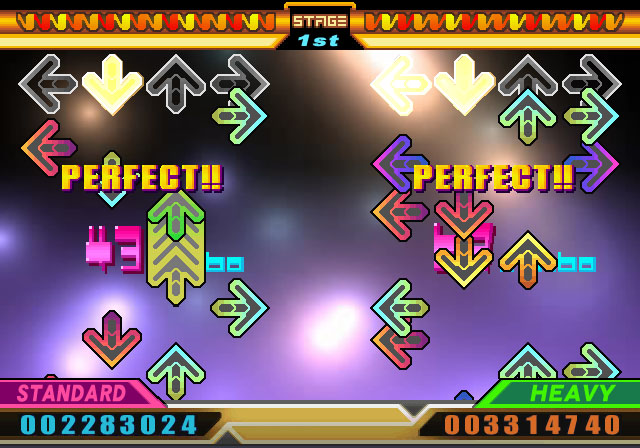
\includegraphics[width=0.43\textwidth]{Figures/dancedancerevolution}
  \end{center}
  \caption{Screenshot from Dance Dance Revolution, an example of a rhythm music game \cite{DDR}.}
\end{wrapfigure}

A music video game can be defined as a type of game that uses music or rhythm as an integral part of gameplay. This may involve pressing buttons in time with a song, whether on a conventional controller, and instrument controller or some kind of dance mat, singing into a microphone or creating original music. Players can often perform different parts of the same song together in local multiplayer games or over the Internet, providing enjoyable social experiences \cite{mvgdef}.

Some games exhibit a sandbox style that encourages a free-form gameplay approach whereas other a hybrid style, which combines musical elements with more traditional genres, for example puzzle games or shooters. 

Below we will briefly go over different types of music video games that can be found on the market.




\subsection{Music Memory Games}

The goal of the music memory game is to score player on their musical memory. Music track is presented to the user who then has to provide an appropriate response to each prompt from the game. Games may be based on different primary musical aspect (whether it is the rhythm, pitch or volume). However, a vast majority of the releases available on the market are rhythm-based.

\begin{figure}
        \centering
        \begin{subfigure}[b]{0.48\textwidth}
                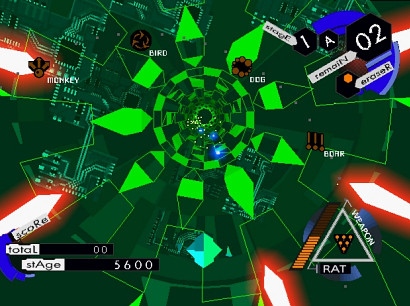
\includegraphics[width=\textwidth]{Figures/is}
                \caption{is - Internal Section - an example of a generative hybrid music game \cite{is}.}
                \label{fig:is }
        \end{subfigure}%
        ~ %add desired spacing between images, e. g. ~, \quad, \qquad, \hfill etc.
          %(or a blank line to force the subfigure onto a new line)
        \begin{subfigure}[b]{0.48\textwidth}
                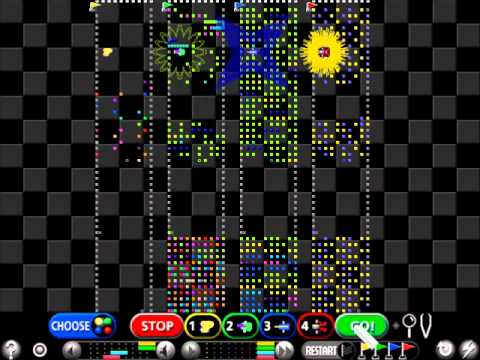
\includegraphics[width=\textwidth]{Figures/simtunes}
                \caption{SimTunes - an example of a free form music game \cite{simtunes}.}
                \label{fig:simtunes}
        \end{subfigure}
          \caption{Examples of music video games.}
        ~ %add desired spacing between images, e. g. ~, \quad, \qquad, \hfill etc.
\end{figure}


Rhythm games typically focus on dance or the simulated performance of musical instruments, and require players to press buttons in a sequence dictated on the screen. Doing so causes the game's protagonist or avatar to dance or to play their instrument correctly, which increases the player's score \cite{rhythmgame}. An example of such games could be Guitar Hero or Dance Dance Revolution.


\subsection{Free Form Music Games}

In free form music games, the main task of the user is to create content. This form of music game is often compared to non-game music synthesisers. Free form music games are somewhere between generative hybrid music games and non-game utilities, depending on the degree to which their gameplay relies on a driving underlying plot-line. An example of such game could be SimTunes, where the user is painting a picture using large pixels and each color represents a musical note. 


\subsection{Hybrid Music Games}

Hybrid music games are characterised by substantial and meaningful interactions between a player and the music game in a game that apparently belongs to a non-musical genre. This type of games can be further split into two sub-types.


Generative music video games make use of user’s actions. By monitoring interaction with the surroundings in the game, the mechanism generates sounds that are then integrated into the soundtrack, permitting the player’s direct interaction with the score. This encourages the creation of a synesthetic experience — when upon stimulation of one sense others activate, causing an involuntary experience. An example of such game could be Rez, which is a simple rail shooter. However, thanks to integrating sounds generated by player completing the normal task of rail-shooting, the score is dynamic.

Reactive music games, in contrast to generative one, employ music to determine the gameplay. In such games, the player takes cues from soundtrack to devise his gameplay. For example, iS - internal section, uses the music to determine the dynamic of the non-musical components of the game.

\begin{figure}
        \centering
        \begin{subfigure}[b]{0.48\textwidth}
                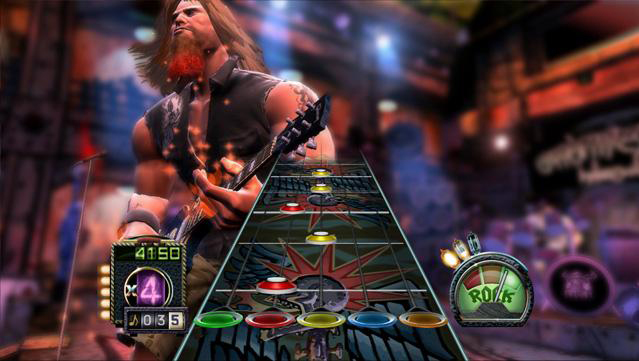
\includegraphics[width=\textwidth]{Figures/guitarhero}
                \caption{Screenshot from Guitar Hero - player is attempting to play a song \cite{ghscreen}.}
                \label{fig:Guitar Hero screenshot}
        \end{subfigure}%
        ~ %add desired spacing between images, e. g. ~, \quad, \qquad, \hfill etc.
          %(or a blank line to force the subfigure onto a new line)
        \begin{subfigure}[b]{0.48\textwidth}
                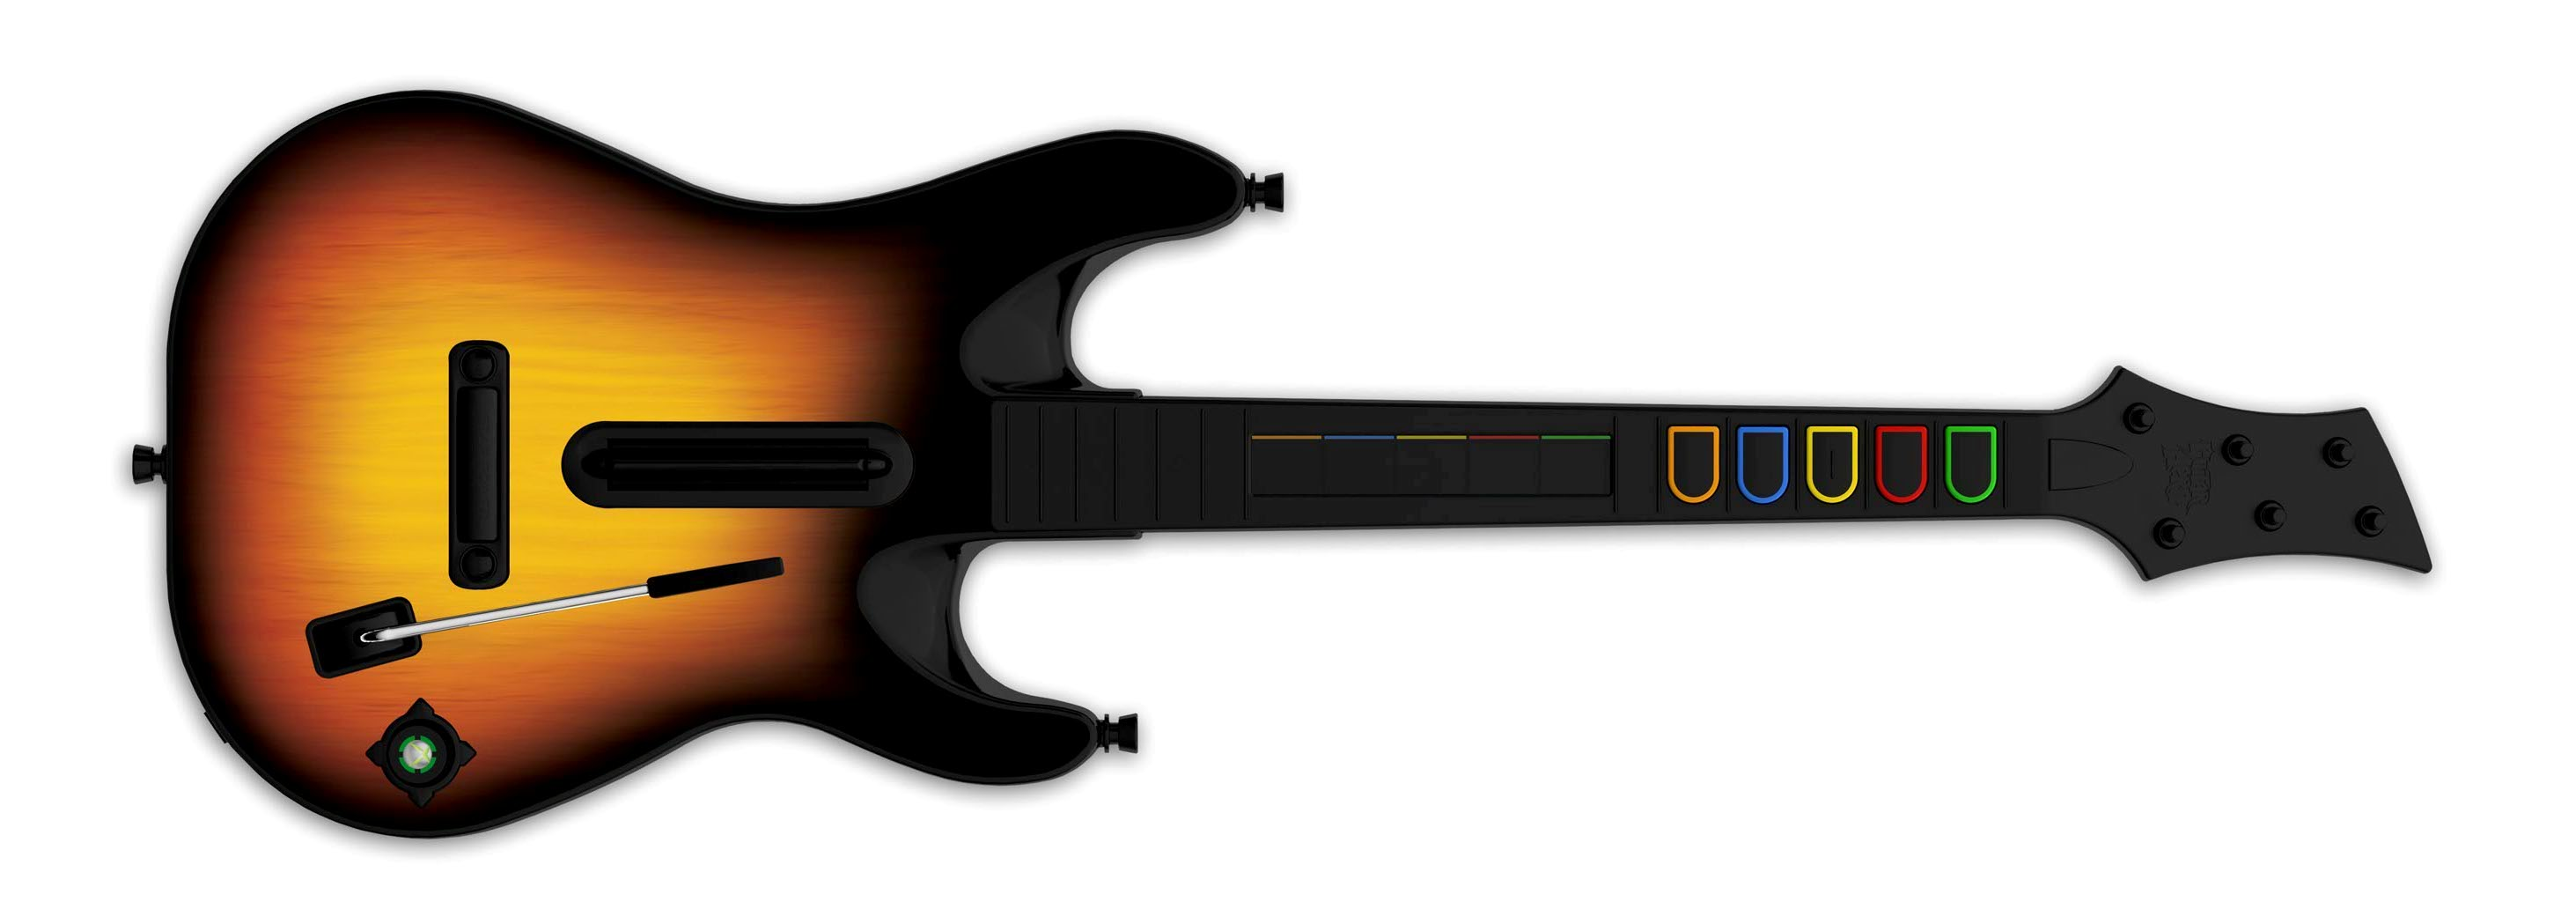
\includegraphics[width=\textwidth]{Figures/controller}
                \caption{A guitar shaped controller used in the game \cite{controller}.}
                \label{fig:Controller}
        \end{subfigure}
          \caption{Guitar Hero components}
        ~ %add desired spacing between images, e. g. ~, \quad, \qquad, \hfill etc.
\end{figure}


\section{Case Study - Guitar Hero}

Guitar Hero is one of the most popular franchises in the history of music games. The first of the series was published in 2005 by RedOctane and Harmonix. In the games, players instrument-shaped game controllers to simulate playing the instruments across numerous rock music songs. It is widely considered a highly entertaining game fully embracing the rhythm-based music game.


\subsection{The Controller}


Rather than a typical gamepad, Guitar Hero uses an instrument-shaped controller (guitar in the earlier releases, bass, microphone and drums in more recent ones). Playing the game with the guitar controller simulates playing an actual guitar, except it uses five coloured "fret buttons" and a "strum bar" instead of frets and strings, and an analogous mapping for the other instruments. They incorporate most of the real life techniques and motions that an instrumentalist would perform on a real instrument.


\subsection{The Gameplay}

The actual game itself works exactly as many other music titles do. At the bottom of the screen, a number of (varying depending of level of difficulty) buttons is shown. In each attempt, a series of notes moves across the screen and when a note aligns with a button, player is supposed to press a corresponding button, gaining points depending on the accuracy. If the player failed to achieve a certain amount of notes — his performance meter stays low for a longer time, he loses the game.

However, there are a couple minor improvements that Harmonix has made to the general music game formula. By acing certain notes in a song, a player is able to build up Star Power, which when unleashed, doubles up current point multiplier. Star Power also adds a bit of a strategic element - player not only earns more points when it is activated, but he can also raise your performance meter faster, enabling him to last longer when encountering a trickier part of a song.


\subsection{The Critique}

Without a doubt, Guitar Hero features a great selection of music. However, there will always be tracks missing, regardless of how many versions of Guitar Hero are released. People have different tastes and limiting a game to a set of tracks that everybody is supposed to enjoy is a really hard task. 

Some more advanced users familiar with Computer Science attempted to transcribe songs and to create new levels. However, this process is really difficult, especially for non computer scientists, discouraging an average user from fully making use of game’s capabilities. The producers, seeing the tendency, started releasing the in-app purchases to enable the players to extend their library and thus, keep the users. 

Implementing a feature of uploading some music preferred by the player would definitely improve user satisfaction. However, this might have not been achieved yet as the task itself is quite complex. Moreover, enabling the users to load in some music would deprive the company of their income sources.

\vspace{30pt}

\section{Introduction to Melody Extraction}

For a long time people were researching ways of estimating the fundamental frequency, be it with monophonic music recording or multi-pitch estimation. Melody extraction differs from both of those problems — unlike monophonic pitch estimation it handles polyphonic tracks and in contrast to multi-pitch estimation, it must also include a mechanism for source identification, to spot the voice carrying the melody within the polyphony.
To be able to evaluate the performance of the new algorithms, annual Music Information Retrieval Evaluation eXchange (MIREX) has been running since 2005. In this campaign, different models are evaluated against the same sets of music collections in order to obtain a quantitative comparison between methods and assess the accuracy of the current state-of-the-art in melody extraction \cite{comparison}.


\subsection{Melody}

The concept of “melody” ultimately relies on the judgment of people listening. This is why it will vary depending on the application context - whether we want to determine symbolic melodic similarity or transcribe a music track. 

In order to have a clear framework to work within, the Music Information Retrieval (MIR) community has adopted in recent years the definition proposed by \cite{melodydef}, “...the melody is the single (monophonic) pitch sequence that a listener might reproduce if asked to whistle or hum a piece of polyphonic music, and that a listener would recognise as being the 'essence' of that music when heard in comparison".

In practice, research has focused on "single source predominant fundamental frequency estimation" — which means a search for a main melody coming from a single sound source throughout the song analysed. As we can see, the subjective element is still present in this description of a melody as there might not be a definite way of deciding what predominant is. However, it fits well with our project’s objective — generating a game level based on changes in the pitch.


\subsection{Polyphonic Music}

Polyphony is a word derived from Greek poluph\={o}nosis meaning more than one sound — a texture consisting of two or more simultaneous lines of independent melody. This can be contrasted with homophony, where musical parts move generally in the same rhythm and one dominant melodic voice is accompanied by chords or monophony, where only one voice is found. 

However, in our case, the term polyphonic will simply refer to any type of music in which two or more notes can be played simultaneously. This can be achieved either by playing in different instruments (for example, voice, guitar and bass) or a single instrument capable of playing more than one more at a time (like a piano).


\subsection{Pitch, Tones, Fundamental Frequency}

Pitch is the most natural way of ordering sounds on a frequency-related scale. If sounds whose frequency is clear and stable enough to be distinguished from noise, they can be compared among  one another as “lower” or “higher”. Pitch is not an objective physical property — it depends on anatomy and physiology of the auditory system, which is a subject of an extensive study called psychoacoustics. 

A semitone is the smallest musical interval commonly used in Western tonal music. Two semitones constitute a tone.

The fundamental frequency $f_{\text{0}}$ is defined as the lowest frequency of a periodic waveform. A harmonic (or a harmonic partial) is any of a set of partials that are whole number multiples of a common fundamental frequency. This set includes $f_{0}$, which is a whole number multiple of itself (1 times itself).

Fundamental frequency can be thought of as the physical property most closely related to perception of pitch. This is why in this context pitch and fundamental frequency can be used interchangeably.


\subsection{Filter}

Any medium through which the music signal passes, whatever its form, can be regarded as a filter. However, we do not usually think of something as a filter unless it can modify the sound in some way. 

A digital filter is a filter that operates on digital signals, such as sound represented inside a computer. It is a computation which takes one sequence of numbers (the input signal) and produces a new sequence of numbers (the filtered output signal) \cite{filters}.


\subsection{Short Time Fourier Transform}

Short-time Fourier transform (STFT), is a signal processing method which is used in analysis of non-stationary signals with statistic characteristics varying with time.
In particular, STFT extracts several frames of the signal to be analysed with a window that moves with time. If we set the window size to be narrow enough, each frame extracted can be viewed as stationary so that Fourier transform can be used. With the window moving along the time axis, the relation between the variance of frequency and time can be identified \cite{STFT}.

The short time Fourier transform of a time-domain signal $y$ is denoted by the matrix $F \times N$, $F$ being the Fourier transform size and $N$ the number of analysis frames.

\section{Main Melody Extraction from Polyphonic Music}
In this section we will go over two different approaches to the problem of main melody extraction from polyphonic music, using source separation and a salience function. Then we will compare both methods to determine which one is more suitable for our project.

\vspace{50pt}

\subsection{Source Separation Based Approach}

\begin{wrapfigure}{r}{0.5\textwidth}
  \vspace{-50pt}

  \begin{center}
    \includegraphics[width=0.48\textwidth]{Figures/durrieudiagram}
  \end{center}
  \caption{Outline of system proposed by Durrieu: X is the STFT of the mixture signal, $p(\Xi|X)$ the posterior probability of a given melody sequence, and $\hat{\Xi} $ the desired smooth melody sequence\cite{durrieu}.}
\end{wrapfigure}


In polyphonic tracks the main melody can be represented by a specific source/filter model. In case of the leading vocal part, the vocal cords are treated as a source and the voice tract as a linear acoustic filter.

In their paper from 2011 \cite{durrieu}, authors presented an algorithm in which they assume that at any given time the signal observed is a mixture of two elementary signals - one corresponding to the main source and one to the background music. Therefore, the signal can be represented in an equation $x(t) = v(t) + m(t)$, where $v(t)$ stands for the source of the main melody and $m(t)$ is the background music. Interestingly, this equation also holds for the short time Fourier transform (STFT)  $X$, $V$ and $M$ respectively: $X = V + M$. The models proposed by Durrieu essentially aim at constraining the shapes of these STFT using temporal and spectral constraints. 


The likelihood of the vocal part V is calculated using two different frameworks. 

The first submission uses the source/filter Gaussian scaled mixture model (GSMM). In this model the source element refers to the excitation of the vocal folds and is therefore linked to the fundamental frequency of the sound $f_{\text{0}}$, while the filter part is characteristic of the vocal tract shape. This space of possibilities is then discretised so that we consider one possible filter frequency response, which is then used to calculate the likelihood of the vocal part knowing the filter and $f_{\text{0}}$.

Fig 2.4. A) shows the diagram of the GSMM model for the main voice part. Each source excitation $u$ is filtered by each filter $k$. The amplitudes for a frame $n$ and for all the couples $(k, u)$ are then applied to each of the output signals. At last a “state selector” sets the active state for the given frame.

The second model was derived from the first one to find a solution that would be more efficient to compute. The authors came up with a formulation that keep the source/filter model within an instantaneous mixture framework (IMM). In this model, for each source a set of filters is defined and at each frame, once every source is filtered and multiplied by a given amplitude, they are all added together.

The background music signal $m(t)$ can be thought of as a mixture of $R$ independent Gaussian sources $m_{r}(t)$. 
Each of the sources is centred and characterised by its power spectral density (PSD), which describes how the power of a signal or time series is distributed over the different frequencies. PSD can be estimated using a Covariance Method.
Due to the linearity of the Fourier transform, $M(f,t)$, the STFT of $m$, is also the instantaneous mixture of the $R$ spectra $M_{r}(f,t)$ of the sources: $M_{r}(f,t)$.
This together with STFT and an amplitude coefficient associated with each source is used to calculate the likelihood for each of the frequency bins. Let $M_{t}(f)$ be the STFT of the background signal at frame $t$ and frequency bin $f$, then we write its likelihood.

\begin{figure}
        \centering
        \begin{subfigure}[b]{0.47\textwidth}
                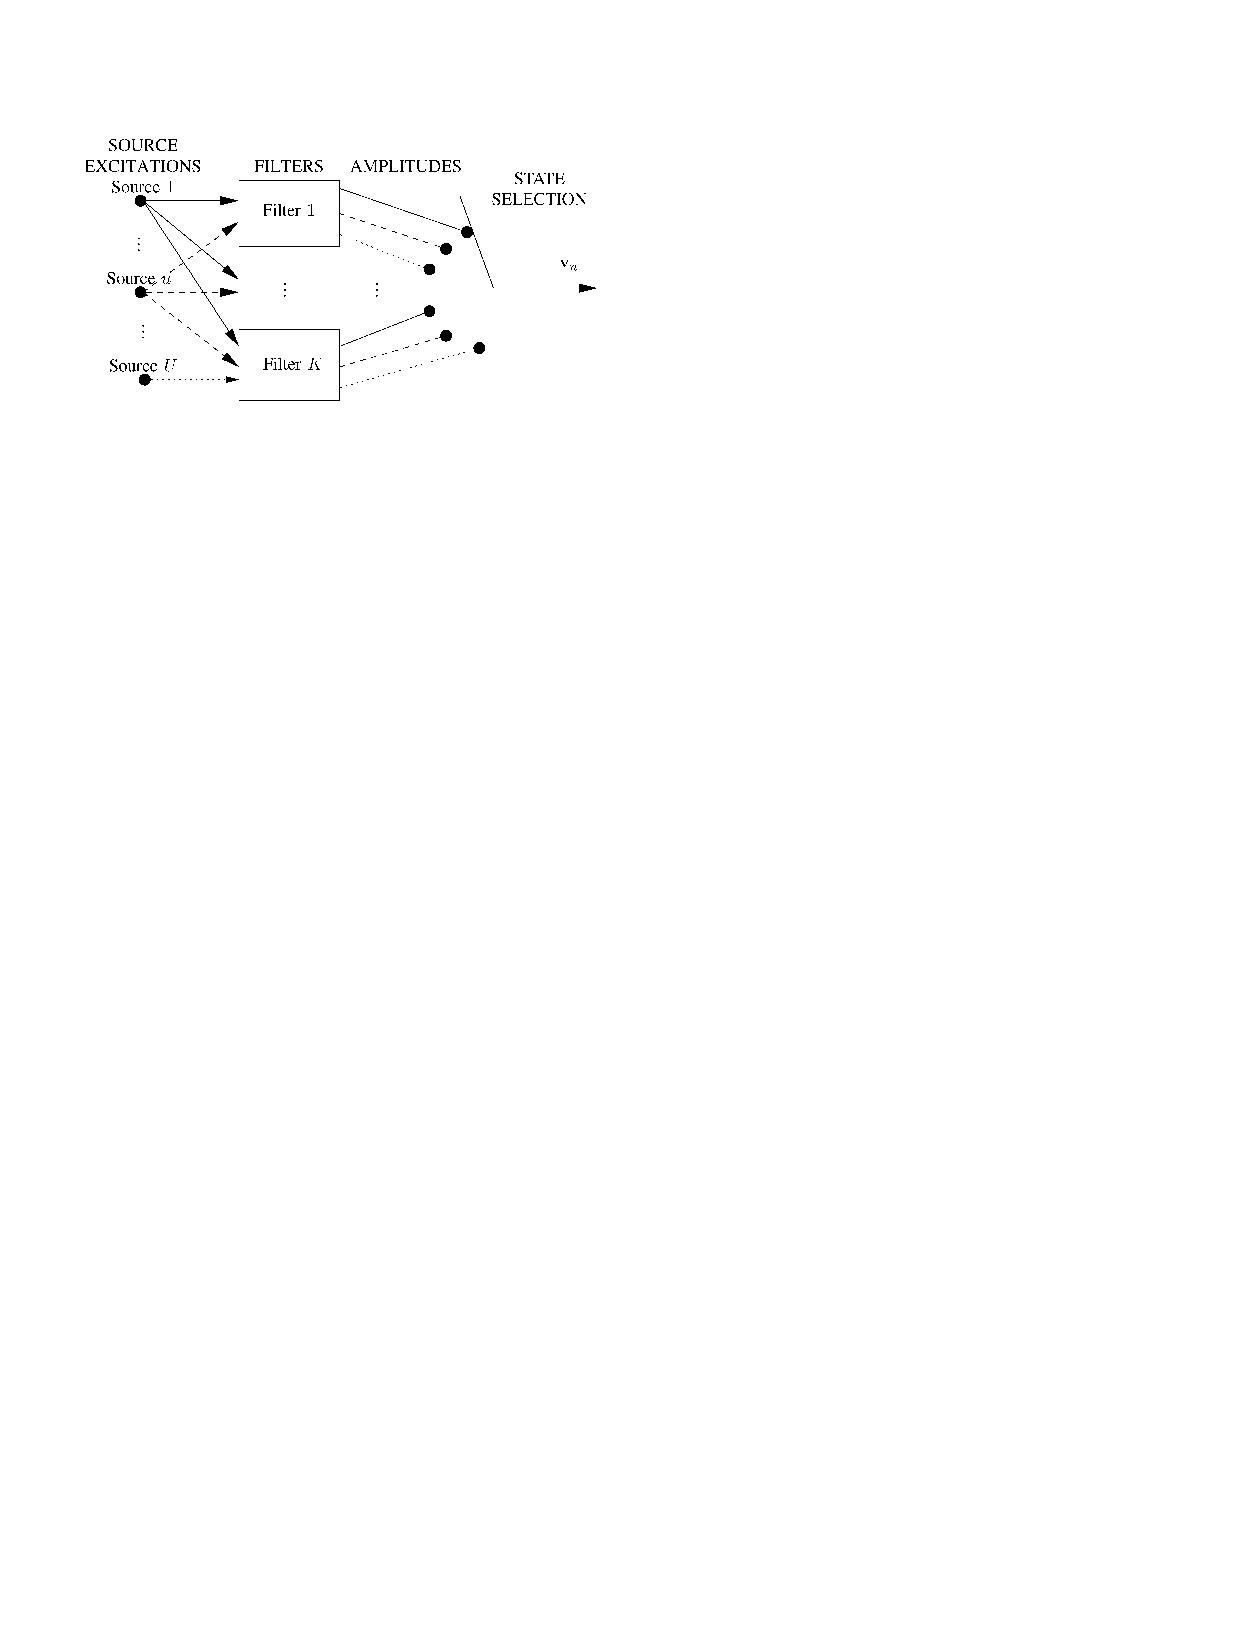
\includegraphics[width=\textwidth]{Figures/gsmm}
                \caption{Schematic principle of the generative GSMM. Each source u is filtered by each filter k. For frame n, the signal is then multiplied by a  given amplitude and a "state selector" then chooses the active state.}
                \label{fig:Guitar Hero screenshot}
        \end{subfigure}%
        ~ %add desired spacing between images, e. g. ~, \quad, \qquad, \hfill etc.
          %(or a blank line to force the subfigure onto a new line)
        \begin{subfigure}[b]{0.47\textwidth}
                \includegraphics[width=\textwidth]{Figures/imm}
                \caption{Schematic principle of the generative IMM. At each frame, all the U sources, each filtered by K filters, are multiplied by amplitudes and added together to produce the leading voice signal.}
                \label{fig:Controller}
        \end{subfigure}
          \caption{Diagram of both models presented in the paper\cite{durrieu}.}
        ~ %add desired spacing between images, e. g. ~, \quad, \qquad, \hfill etc.
\end{figure}

Once the parameters are estimated using the maximum likelihood criterion for each of the model, the Viterbi smoothing of the melody line is applied, obtaining a trade-off between the smoothness of the melody and its global energy in the signal. The Viterbi algorithm is a dynamic programming algorithm for finding the most likely sequence of hidden states – called the Viterbi path – that results in a sequence of observed events \cite{viterbi}.
 
The authors then parametrise the transitions between the possible main melody without disabling jumps from one note to the other. Using Wiener filtering - digital signal processing reducing the noise, using an statistical estimate of the signal using a desired data without such noise, a framework is implemented to separate the source. This way separated signals are obtained. Computing the energy for each frame of the separated main melody and thereafter thresholding allowed to discriminate between spurious notes and true positives.


\subsection{Salience Based Approaches}

\begin{wrapfigure}{r}{0.5\textwidth}
  \vspace{-60pt}

  \begin{center}
    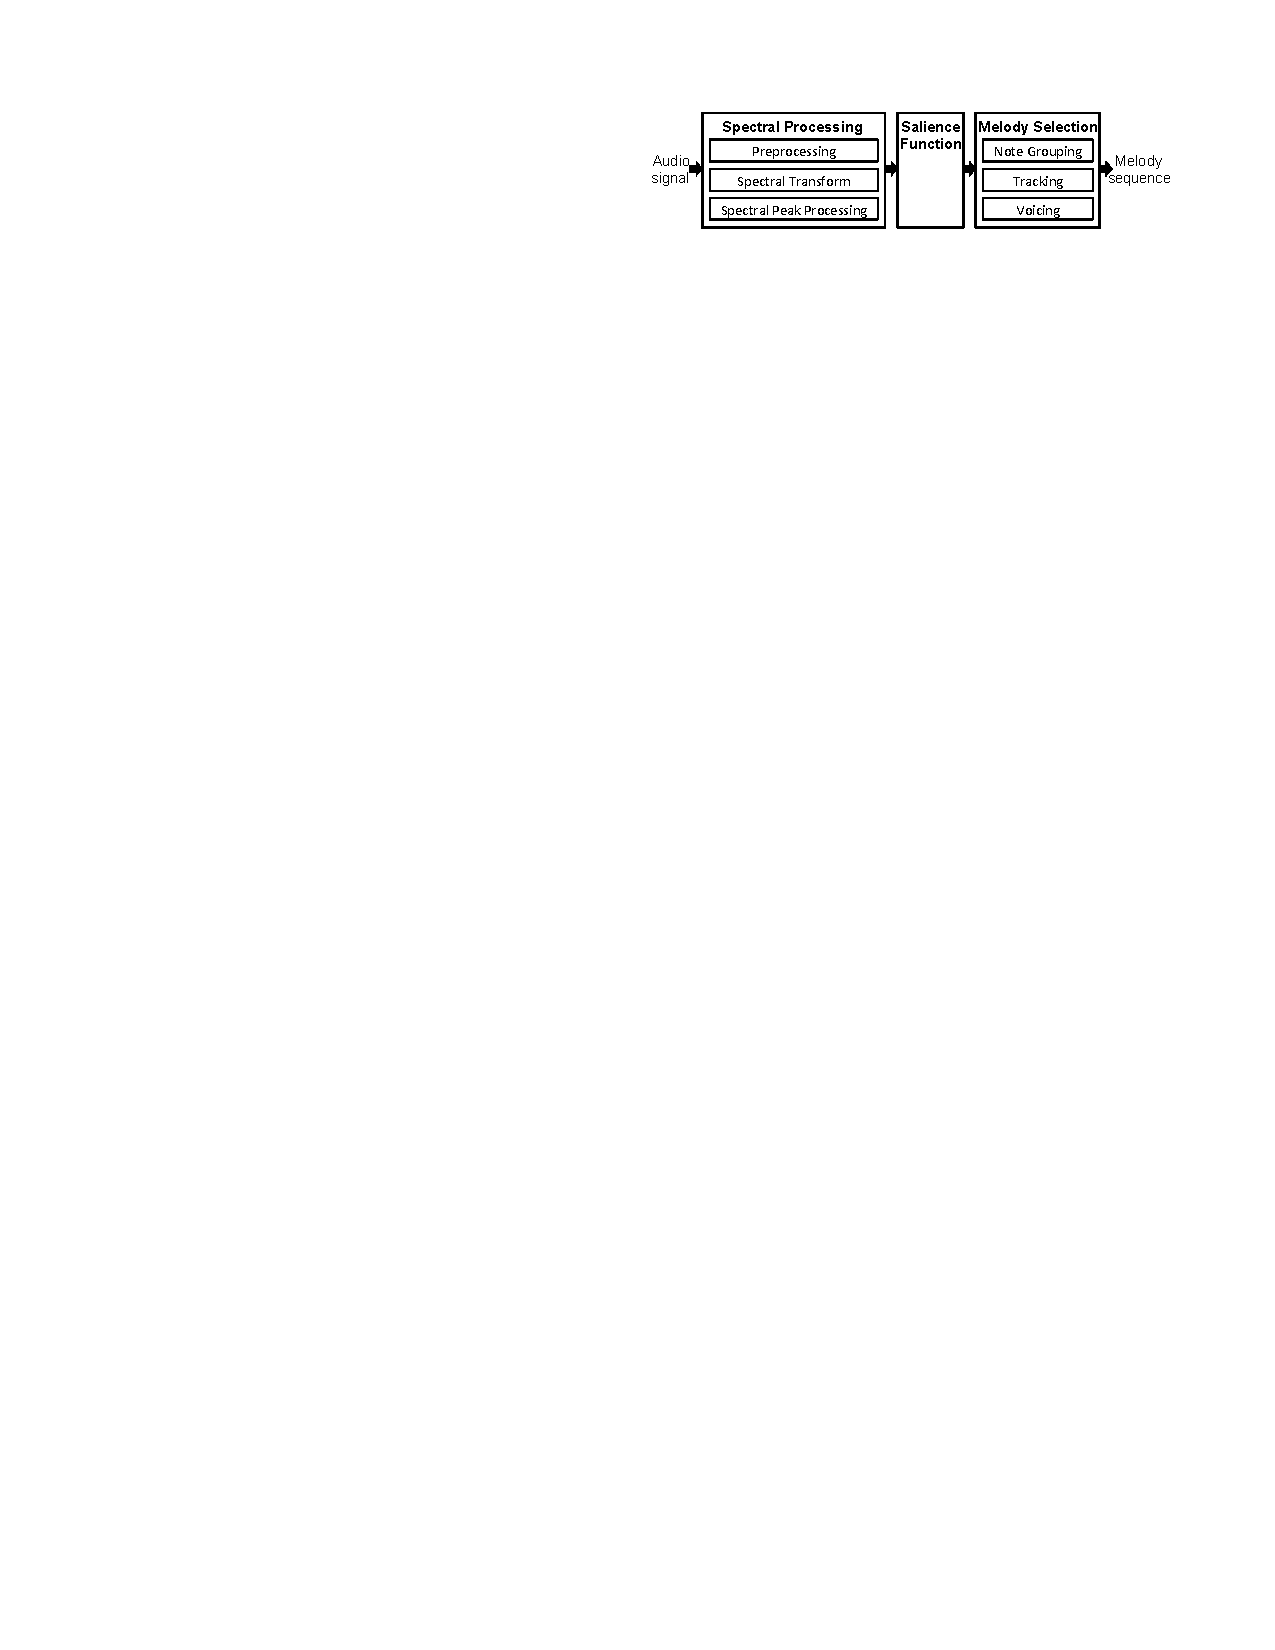
\includegraphics[width=0.48\textwidth]{Figures/salienceoveralldiagram}
  \end{center}
  \caption{Block diagram of four main blocks of the system by Salamon and G\'{o}mez: sinusoid extraction, salience function computation, pitch contour creation and melody selection \cite{comparison}.}
\end{wrapfigure}

This approach has been the most popular so far, with majority of algorithms evaluated at MIREX implementing it. It and can be split into several smaller stages, as seen in Figure 2.5. In particular, a method implemented in paper \cite{salamon} seems to be quite promising.

Usually as a first step, some sort of preprocessing is applied to the audio signal, usually to enhance the frequency content where we expect to find the melody. In particular, Salamon and G\'{o}mez apply an equal loudness filter, which enhances the frequencies to which the human ear is more perceptually sensitive, by taking a representative average of the equal loudness curves and filtering the signal by its inverse. 

This stage is followed by spectral transform — the signal is chopped into time frames and a transform function is applied to obtain a spectral representation of each frame.
This is achieved by applying the Short-Time Fourier Transform given by:

\begin{equation}
X_{l}(k) = \sum_{n=0}^{M-1} w(n) \times x(n + lH) e^{-j\frac{2 \pi}{N}kn}
\end{equation}

with a window length of 46.4ms. Here, $x(n)$ is the time signal, $w(n)$ the windowing function, $l$ the frame number, $M$ the window length, $N$ the FFT length and $H$ the hop size. Thanks to choosing a relatively small hop size, Salamon and G\'{o}mez achieve sufficient frequency resolution to identify different notes while maintaining adequate time resolution to track pitch changes in the melody over a short time. 

Having done this, we move to frequency/amplitude correction, where the spectral peaks are detected and used to construct a salience function. To avoid a relatively large error in the estimation of the peak frequency caused by binning them in the process of FFT, peak’s instantaneous frequency and amplitude are calculated. 

\begin{wrapfigure}{l}{0.5\textwidth}
  \vspace{-30pt}

  \begin{center}
    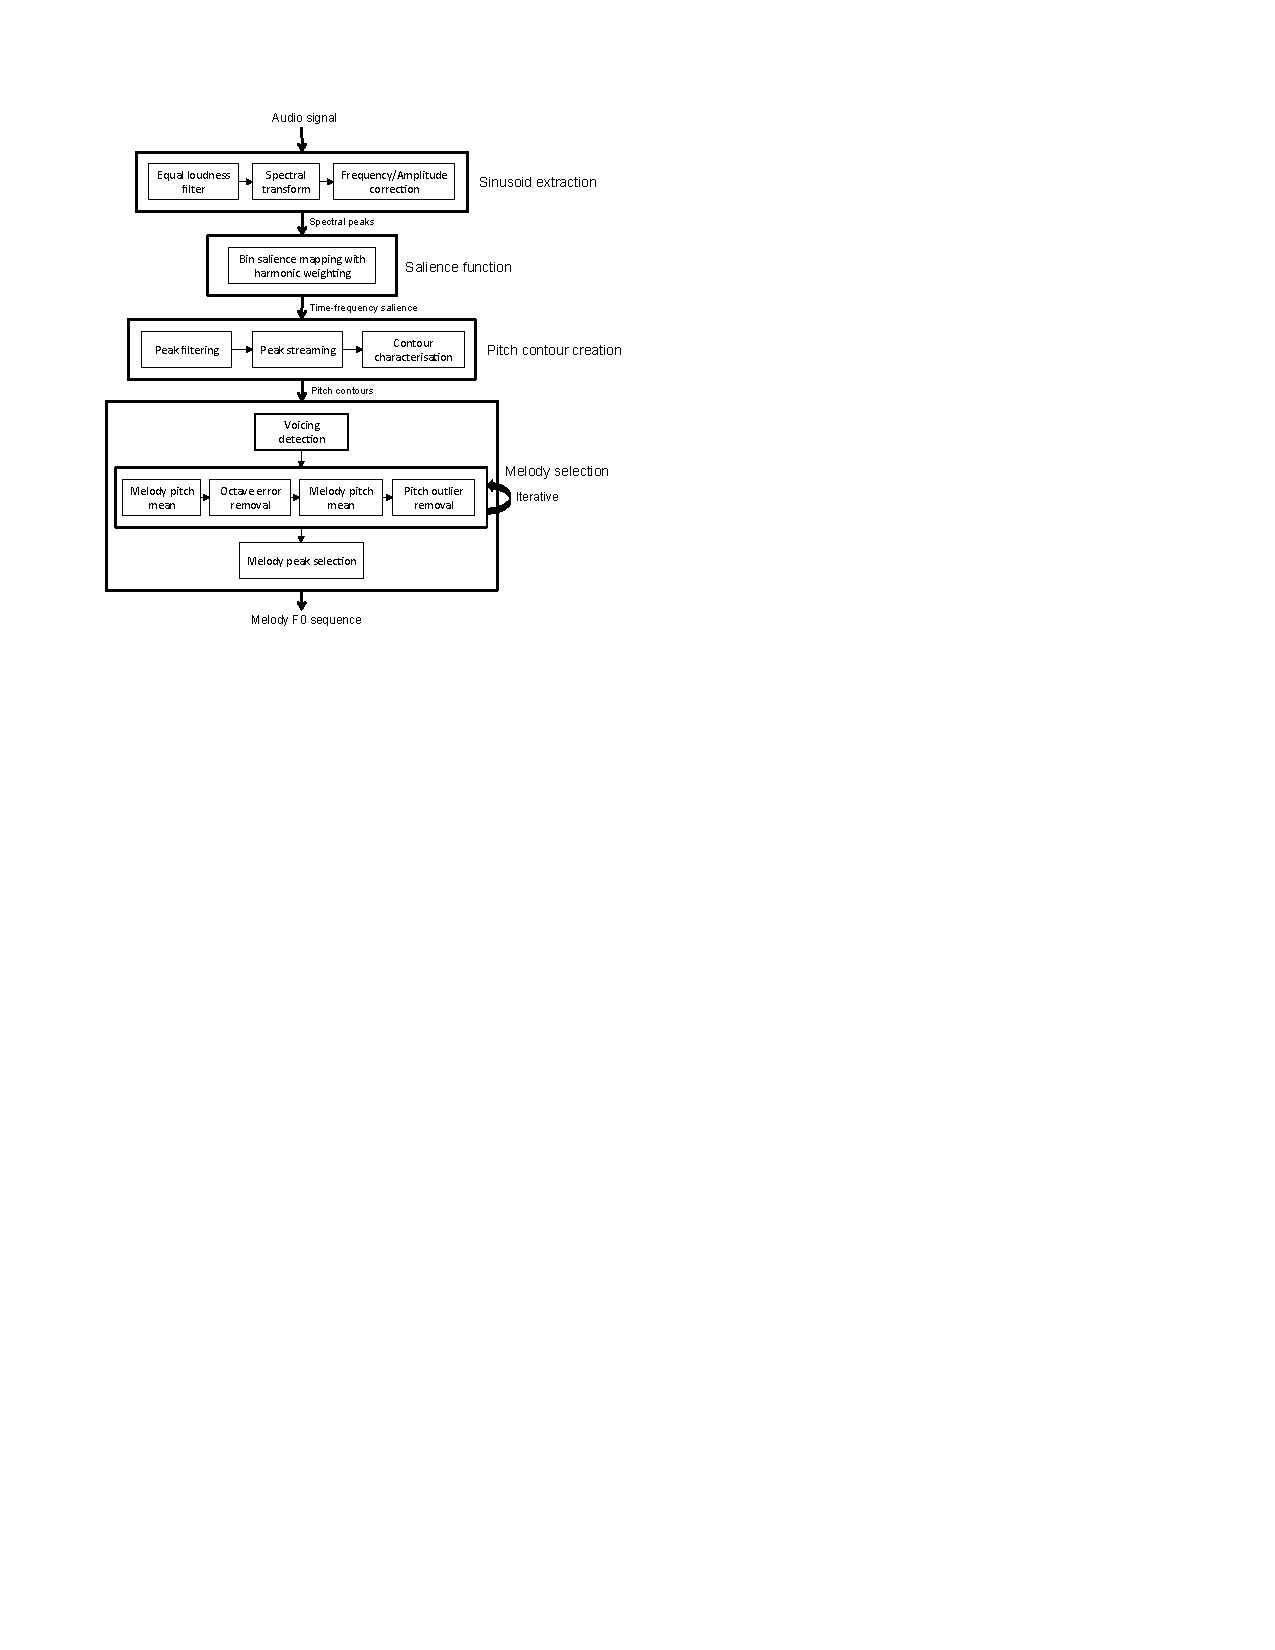
\includegraphics[width=0.48\textwidth]{Figures/salamon4blocksdiagram}
  \end{center}
  \caption{Block diagram of four main blocks of the system by Salamon and G\'{o}mez: sinusoid extraction, salience function computation, pitch contour creation and melody selection \cite{salamon}.}
\end{wrapfigure}

As we can see in figure 2.6, those three steps constitute the spectral processing. But at the core of the salience based algorithms lies the multi-pitch representation, i.e. the salience function — a representation of pitch salience over time. The peaks of this function form the $f_{0}$ candidates for the main melody. In the algorithm described by Salamon and G\'{o}mez, this computation is based on harmonic summation, where the salience of  a given frequency is computed as a sum of the weighted energies found at harmonics (integer multiples) of that frequency. Using only the peaks for the summation allows the authors to discard less reliable values and apply further frequency corrections. 

The salience function presented in the paper covers a pitch range of nearly five octaves from 55Hz to 1.76kHz.

Peaks of the salience function at each frame are now potential $f_{0}$ of the main melody. At this point some methods for melody extraction attempt to track the melody. However, Salamon and G\'{o}mez filter out the non-salient peaks, first by comparing them to the highest peak in the frame and then to a value computed using salience mean and standard deviation of all remaining peaks (in all frames). Now the peaks are grouped into pitch contours - time and pitch continuous sequences of salience peaks as shown in Figure 2.7.


\begin{figure}[h!]
  \centering
    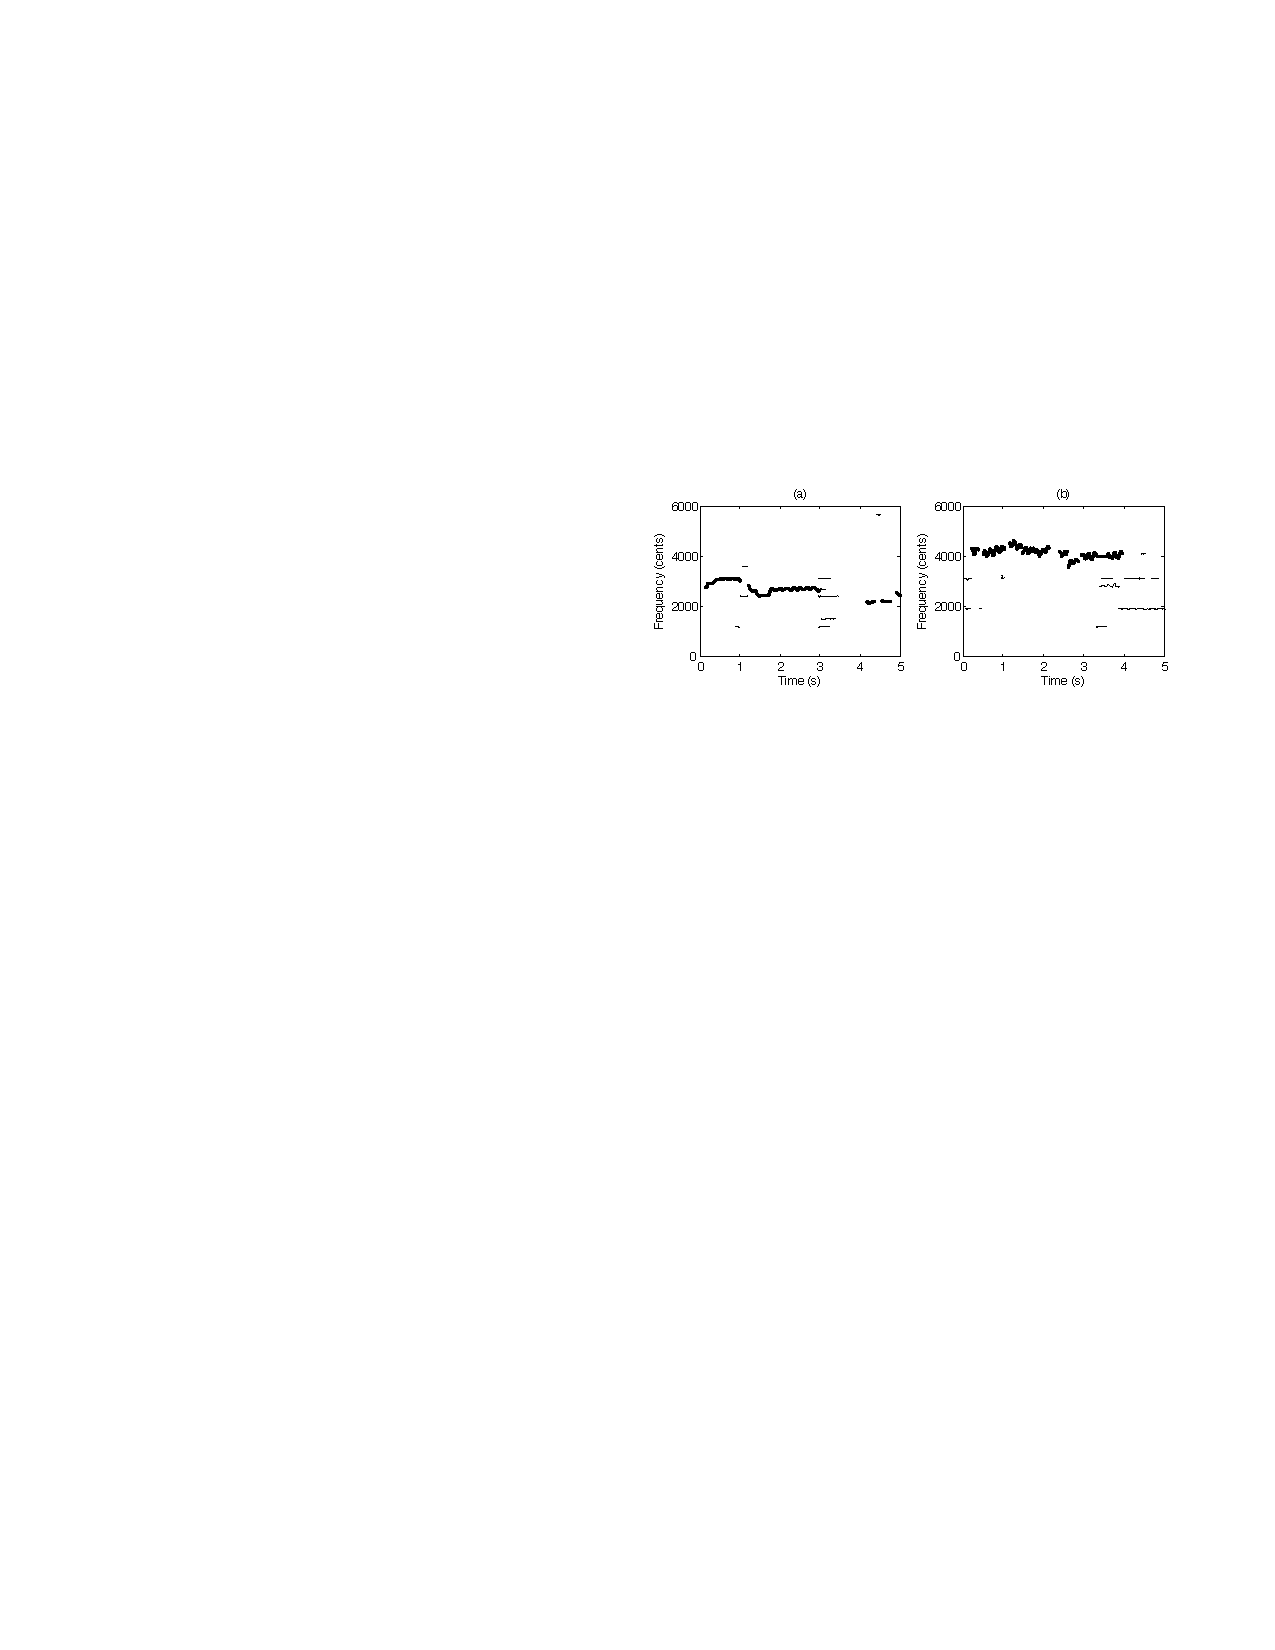
\includegraphics[width=0.7\textwidth]{Figures/pitchcontour}
      \caption{Pitch contours generated from excerpts of (a) vocal jazz and (b) opera. Melody contours are highlighted in bold\cite{salamon}.}

\end{figure}

Having created the pitch contours, Salamon and G\'{o}mez are faced with the task of determining which one belongs to the main melody. The authors define features based on contour pitch, length and salience.

Given the peaks of the salience function, we now have to determine which pitch values belong to the melody. This process is initiated by grouping peaks into continuous pitch contours, out of which a melody is selected later. 

The next main block in this algorithm shown in Figure 2.6 is the melody selection which is comprised of three steps: voicing detection, octave error minimisation/pitch outlier removal, and final melody selection.
As the name suggests, the aim of the voicing detection is to determine when the melody is present.


To filter out these contours Salamon and G\'{o}mez take advantage of the contour mean salience distribution.
By setting the threshold to a value slightly below the average contour mean salience of all contours in the excerpt $C_{s}$, we can filter out a considerable amount of non-melody contours. The authors define the following voicing threshold $\tau_{v}$ based on the distribution mean $C_{s}$ and its standard deviation $\sigma_{\overline{s}}$:
\begin{equation}
\tau_{v} = C_{s} - v \times \sigma_{\overline{s}}
\end{equation}

The parameter $v$ determines the lenience of the filtering - a high $v$ value might keep the false melody contours and a low value might filter out the melody contours.

It is also important to note that detecting certain characteristics in the contour increases a probability of it being the melody contour, for example in case of detecting a vibrato -  a regular, pulsating change of pitch, used to add expression to vocal and instrumental music. \cite{vibrato}

Next step in the melody selection described by Salamon and G\'{o}mez in their paper is octave errors and pitch outliers removal.  

In particular, the octave errors are the main sources of errors in melody extraction systems, when a multiple or sub-multiple of $f_{0}$ is reported as the main melody. 

To detect such errors, contour trajectories are compared by computing distance between their values on a per-frame for the region they overlap in and computing the mean over this region.
If the mean distance is within $1200\pm50$ cents, the contours are considered octave duplicates.

Secondly, Salamon and G\'{o}mez use the relationship between neighbouring contours (in time) to decide which of the duplicates is the correct one. Their approach is based on two assumptions: firstly, that most (though not all) of the time the correct contour will have greater salience than its duplicate (the salience function parameters were optimised to this end). Secondly, that melodies tend to have a continuous pitch trajectory avoiding large jumps, in accordance with voice leading principles.

The method iteratively computes the $\overline{P(t)}$ - pitch trajectory that represents the time evolution of the melody's pitch.
It then detects and removes an octave duplicate as well as  the "pitch outliers” – contours more than one octave above or below the pitch mean and then it is recalculated. Authors empirically discovered that 2 iterations of this process are enough to get a good approximation of the true trajectory of the melody, which is then passed to the final stage of the model - the final melody selection.

At this stage, there is often only one peak to be chosen as the main melody. When there is still more than one contour present in a frame, the melody is selected as the peak belonging to the contour with the highest total salience $C_{\sum s}$. If no contour is present the frame is regarded as unvoiced.

\subsection{Comparison of both approaches}

In their paper \cite{comparison}, authors attempted to compare multiple melody extraction algorithms created since 2005. One of the methods, used also by MIREX, is based on the per-frame comparison, considering different measures:


\begin{description}
\item[Voicing Recall Rate] - the proportion of frames labeled as melody frames in the ground truth that are estimated as melody frames by the algorithm.
\item[Voicing False Alarm Rate] - the proportion of the frames labeled as non-melody in the ground truth that are mistakenly estimated as melody frames by the algorithm.
\item[Raw Pitch Accuracy] - the proportion of melody frames in the ground truth for which $f_{\tau}$ is considered correct (i.e. within half a semitone of the ground truth). 
\item[Raw Chroma Accuracy] - as raw pitch accuracy, except that both the estimated and ground truth $f_{0}$ sequences are mapped onto a single octave. This gives a measure of pitch accuracy which ignores octave errors.
\item[Overall Accuracy] - this measure combines the performance of the pitch estimation and voicing detection tasks to give an overall performance score for the system. It is defined as the proportion of all frames correctly estimated by the algorithm, where for non-melody frames this means the algorithm labeled them as non-melody, as for melody frames the algorithm both labeled them as melody frames and provided a correct $f_{0}$ estimate for the melody (again, within half a semitone of the ground truth).
\end{description}


\begin{figure}[h!]
  \centering
    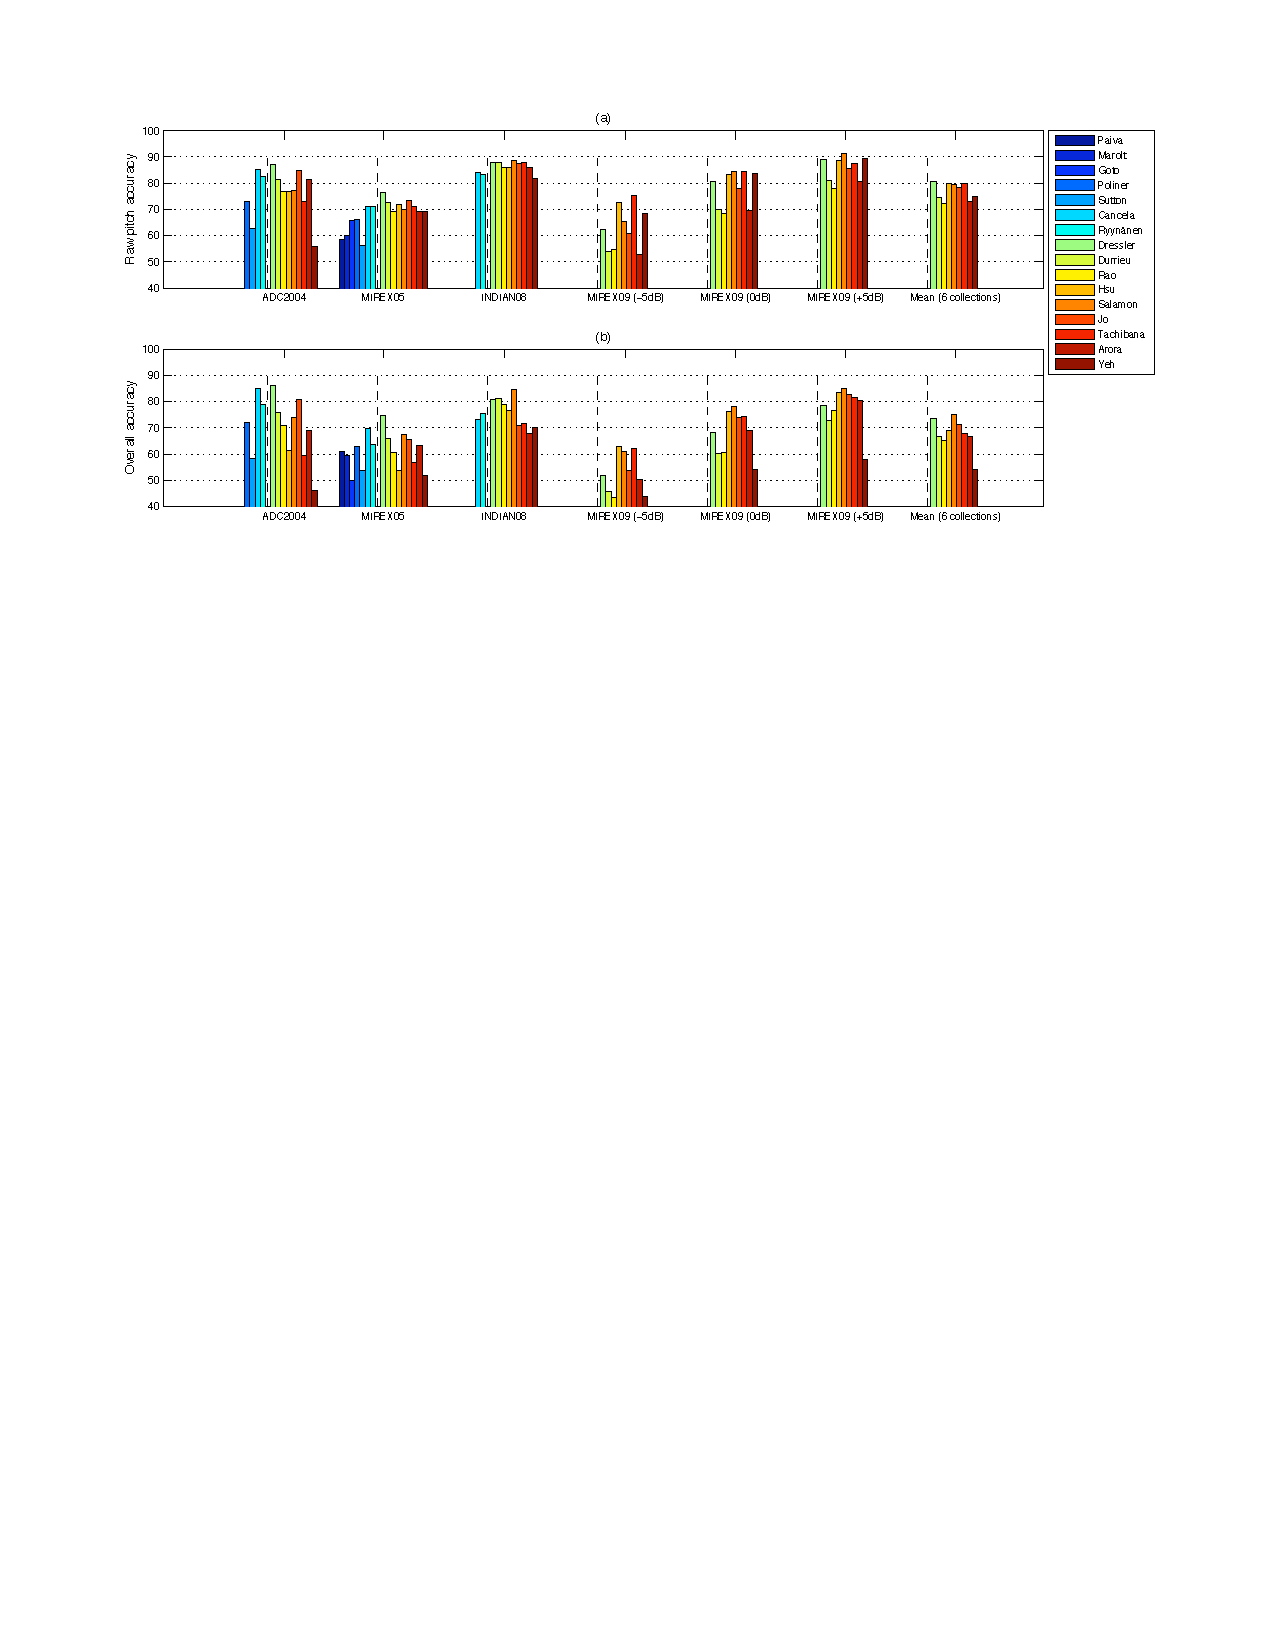
\includegraphics[width=\textwidth]{Figures/comparisonall}
      \caption{a) Raw pitch accuracy and b) overall accuracy obtained in MIREX by 16 melody extraction algorithms evaluated in \cite{comparison}. The vertical dashed line separates the algorithms that were only evaluated on some collections (left of the line) from those evaluated on all six collections (right of the line)\cite{comparison}.}
\end{figure}


In Figure 2.8. the authors presented results obtained by the algorithms evaluated at MIREX. To get a general idea of the performance of the algorithms, it is sufficient to focus on two evaluation measures.
The raw pitch accuracy, presented in Figure 2.8 a) represents how well the algorithm tracks the pitch of the melody. The overall accuracy on the other hand, as shown in Figure 2.8 b), combines this measure with the efficiency of the algorithm's voicing detection, meaning the voicing-related measures are also reflected in this measure.

As we can see, some collections are generally hard to analyse (for example MIREX09 -5db), in general the collections yield different results for different algorithms. This allows us to spot pros and cons of each approach investigated.

We can also notice that the raw pitch accuracy gradually improved from 2005 to 2009, after which it stayed relatively unchanged. Overall we can see that the average pitch accuracy over a collection lies between 70-80%.

On the other hand, when it comes to overall accuracy, the performance goes down compared to the raw pitch accuracy for all algorithms due to voicing detection being factored into the results. The importance of this step depends on the intended use of the algorithm. Generally, the overall accuracy results lie between 65-70%.

Finally, an important factor in assessment of an algorithm is its complexity. While deriving O-notation is too complex for some of the algorithms, generally it is observed that algorithms involving source separation are significantly more computationally complex than salience based approaches Unfortunately, there is no specific data provided by Salamon and G\'{o}mez [9] or by Durrieu [5] on their algorithms.

In conclusion, we believe the solution proposed by Salamon and G\'{o}mez is better fitted to the purpose of this project. The paper presents it in a much clearer way and, what is most important, it outperforms the one created by Durrieu significantly, as seen in Figure 2.8.. In addition to this, according to tendency it is less computationally expensive, which is quite important when it comes to game designing as we do not want to keep the user waiting for a long time for his level to generate and load.

\section{Mood Detection}
It is well known that music can convey emotion and modulate mood. That is why the relation between musical sounds and their influence on the listener’s emotion has been well studied.

One of the first publications on emotion detection in music is credited to Feng, Zhuang, and Pan \cite{moodold}. They employ Computational Media Aesthetics to detect mood for music information retrieval tasks. The two dimensions of tempo and articulation are extracted from the audio signal and are mapped to one of four emotional categories; happiness, sadness, anger, and fear. 
After that, feature called relative tempo is calculated, and after the mean and standard deviation of the feature called average silence ratio in the presented computational articulation model are calculated, a simple Back Propagation neural network classifier is trained to detect mood.

In publication by Yang, Lin, Su and Chen \cite{mood}, the authors presented a tool which recognises a mood in a musical track, allowing a user to then choose the song they want to play by deciding on emotions it is supposed to represent.
Specifically, the authors formulate music emotion recognition as a regression problem to predict the arousal and valence values (AV values) of each music sample directly.

Potentially, the second approach described seems more appropriate for our project as it allows for better granularity in the melody emotion detection and, hence, wider variety of changes in the game's environment. However, this area of the project is left to be further researched.


\section{Level Generation}
It is not really surprising that there is no current literature on the problem of automatically generating Guitar Hero buttons given an arbitrary piece of music.
However, we believe an algorithm can be developed where the buttons can be mapped to the $f_{0}$ in the main melody extracted by main melody extraction algorithm. 
% Project Plan

\chapter{Project Plan (1-2)} % Main chapter title

\label{Chapter3} % For referencing the chapter elsewhere, use \ref{Chapter3} 

\lhead{Chapter 3. \emph{Project Plan}} % This is for the header on each page - perhaps a shortened title

%----------------------------------------------------------------------------------------


% Evaluation

\chapter{Results and Evaluation} % Main chapter title

\label{Chapter6} % For referencing the chapter elsewhere, use \ref{Chapter4} 

\lhead{Chapter 6. \emph{Results \& Evaluation}} % This is for the header on each page - perhaps a shortened title

%----------------------------------------------------------------------------------------

Success of any project or product depends on many factors - the performance, design, innovation and design. Each of the elements it consists of contribute to at least one of them. 
In this chapter we evaluate our project in attempt to assess its success.

First, we focus on quantitative analysis. We present the results of testing and validating of our neural network for music emotion prediction using fresh and unseen data and contrast them with existing literature. Then we move on to evaluation of the boundary detection system by comparing the performance and accuracy it yields with two other algorithms. Finally, we examine the results of the labelling algorithm.

Last, but not least, we move on to user experience research. We go over user testing and its outcome, as well as how it was used to further improve our game. 

\vspace{10pt}

\section{Evaluation of Mood Detection system}

\begin{figure}[t]
    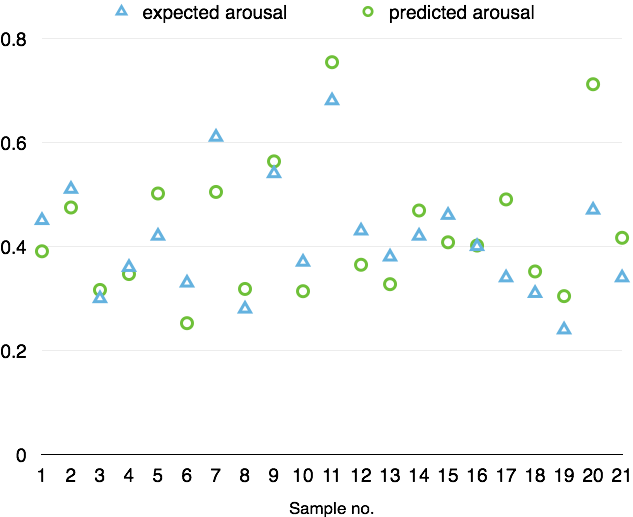
\includegraphics[width=0.7\textwidth]{Figures/finalarousal}
    \centering

  \caption{A plot of the expected and predicted .}
  \label{fig:anneval}
\end{figure}


We designed our neural networks to as means of calculating valence and arousal ratings of songs using audio features we extract. 

To evaluate its performance we have to have a way of telling how successful it is in guessing the values. To achieve this, we activated the network on 21 unseen music tracks that we knew valence and arousal values of and gathered the output network produced for it. Then, we computed the root mean square error between the ground truth ratings and network-predicted outputs across all segments of all the test melodies. The network's performance total RMSE was 0.08895 on scale from 0 to 1 or 9\%. The plot of the expected and predicted values can be seen in Figure \ref{fig:anneval}.

In contrast, in their paper \cite{vempala} Vempala and Russo trained a neural network with 1.14 error on scale 1 to 9, or 14.3\%.

If we look at the two predicted values separately, the coefficient of determination for the arousal reached 59.24\% and 40.34\% for valence.

In comparison, Yang and Lin \cite{mood} achieved a lower success rate, as their $R^2$ scored 58.3\% for arousal and 28.1\% for valence. 


\begin{figure}[t]
    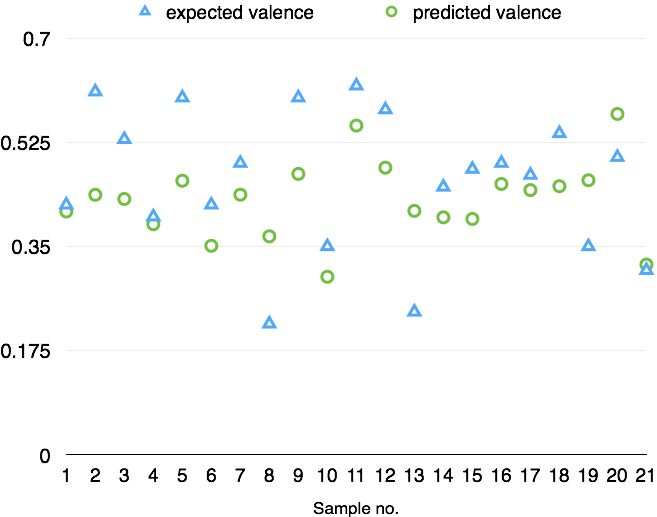
\includegraphics[width=0.7\textwidth]{Figures/finalvalence}
    \centering

  \caption{A plot of the expected and predicted valence.}
  \label{fig:anneval}
\end{figure}


Results from the static network indicate that a network can be trained to identify statistical consistencies across audio features abstracted from music and satisfactorily predict valence/arousal values that closely match mean participant ratings.


\begin{table}
\begin{center}
\begin{tabular}{| c | c | c | c | } \hline 
 expected arousal & expected valence & predicted arousal & predicted valence \\ \hline \hline

0.45  & 	0.42  &  0.390444 &  0.408524   \\ \hline
0.51	&  0.61  &  0.474538 & 0.436625   \\ \hline
0.3    &  0.53  &  0.316230 & 0.429643   \\ \hline
0.36	&  0.4    &  0.346713 & 0.387249   \\ \hline
0.42	&  0.6    &  0.501414 & 0.460295   \\ \hline
0.33	&  0.42  &  0.252398 & 0.350910  \\ \hline
0.61	&  0.49  &  0.504392 & 0.436785   \\ \hline
0.28	&  0.22  &  0.318096 & 0.366836   \\ \hline
0.54	&  0.6    &  0.563120 & 0.471717   \\ \hline
0.37	&  0.35  &  0.313782 & 0.298909   \\ \hline
0.68  &  0.62  &  0.753534 & 0.552922   \\ \hline
0.43	&  0.58  &  0.364568 & 0.482194   \\ \hline
0.38	&  0.24  &  0.327288 & 0.409628   \\ \hline
0.42  &  0.45  &  0.468762 & 0.398749   \\ \hline
0.46  &  0.48  &  0.407701 & 0.396029   \\ \hline
0.4    &  0.49  &  0.401469 & 0.454892   \\ \hline
0.34  &  0.47  &  0.490065 & 0.444592   \\ \hline
0.31  &  0.54  &  0.351714 & 0.451086   \\ \hline
0.24  &  0.35  &  0.304314 & 0.461078   \\ \hline
0.47	&  0.5    &  0.711224 & 0.572459   \\ \hline
0.34	&  0.31  &  0.416320 & 0.319491   \\ \hline
\end{tabular}
\caption{Table showing the root mean square error for training the network for given number of nodes in the hidden layer.}
\label{table:rsmetablefinal}
\end{center}
\end{table}



\section{Boundary Detection}

The first towards the evaluation of the segmentation algorithm was to gather the ground truth data to test against. To remove bias caused by personal preferences in music, we sought external sources for help in selection of the tracks. This is why we consulted the top charts created by music magazines and online portals such as Rolling Stone, Billboard, Gibson etc. The full list can be found in \cite{toplists}.

Once we have retrieved the lists with the most popular songs across genres, we selected one song per top list based on our familiarity. Although this might introduced some sort of personal preference into the dataset, it also allowed us to more intuitively create the ground truth data, as the familiarity with a song makes the manual labelling more obvious. For instance, in “Blitzkrieg Bop” by The Ramones, the bridge is repeates as often as verse and chorus, which is bound to introduce confusion to a person who hears the song for the first time and is asked to segment and label it.

In totall, we manually labelled 10 songs:
\vspace{-10pt}
\begin{description}
\itemsep0em 
\item[“The Number of The Beast”] by Iron Maiden (Metal)
\item[“Rock With You”] by Michael Jackson (Soul/R\& B)
\item[“Blitzkrieg Bop”] by The Ramones (Punk Rock)
\item[“This Land is Your Land“] by Woody Guthrie (Folk)
\item[“One More Time”] by Daft Punk (Dance)
\item[“Smooth”] by Santana (featuring Rob Thomas) (Pop)
\item[ “Crazy in Love”] by Beyonce (featuring Jay-Z) (Pop / Rap)
\item["Help!"] by The Beatles (Rock)
\item["Respect"] by Aretha Franklin (R\& B)
\item["Back in the USSR"] by The Beatles (Rock)
\end{description}

For each of the songs, we conducted 5 measurements to manually detect the boundaries. Once we have gathered the data, we averages each bound to create ground truth with reference boundaries and labels.

To be able to fully evaluate the performance of our algorithm in comparison with state-of-the-art solutions already existing, we also gathered data produced by two other algorithms. The first one, described by Foote and Cooper \cite{FooteCooper}, is a classic approach applying a "“checkerboard” kernel over the diagonal of a self similarity-matrix (SSM). The other one is an approach published by Kaiser and Sikora \cite{Sikora}, with use of non-negative matrix factorisation on only one feature. 

We conducted two types of studies to determine the performance of our bound finding algorithm.

First and the most intuitive one is the comparison of amount of boundaries detected. If an algorithm returns a smaller amount of segments it means that most probably its detection system is not sensitive enough - it merges some of bounds into bigger ones. And vice versa - if the algorithm returns more boundaries than the ground truth, it means it picked on song segments that differ in a less obvious way and, hence, its output is too granular.


\begin{table}
\begin{center}
\begin{tabular}{| c | c | c | c | c | } \hline 
Song  								& Ground	& Foote 	&  Kaiser 	& Ours \\ \hline \hline
The Number of The Beast 	&	17			& 	9  			&  15 		&  20   	\\ \hline
Rock With You					&	11			&  9			&  15 		& 17   	\\ \hline
Blitzkrieg Bop 					&	14			&  9  			&  14 		& 14   	\\ \hline
This Land Is Your Land 		&	11			&  9			&  12 		& 7    	\\ \hline
One More Time					&	13			&  9    		&  14 		& 17   	\\ \hline
Smooth								&	14			&  9  			&  14 		& 16  	\\ \hline
Crazy In Love					&	17			&  9  			&  13  		& 16   	\\ \hline
Help!									&	10			&  9		   	&  17 		& 12   	\\ \hline
Respect								&	12			&  9  			&  14 		& 12  	\\ \hline
Back In the USSR				&	15			&  9  			&  13		    	& 14		\\ \hline \hline
RMSE								&	N/A		& 4.98		&  3.08		& 2.95	\\ \hline 

\end{tabular}
\caption{Table showing the root mean square error for training the network for given number of nodes in the hidden layer for the checkerboard algorithm (by Foote, \cite{FooteCooper}), NMF based algorithm (by Kaiser, \cite{Sikora}) and ours.}
\label{table:evalStructureCount}
\end{center}
\end{table}


The results of our investigation can be seen in Table \ref{table:evalStructureCount}. By calculating the root mean square error for outputs of every algorithm, we noticed that our algorithm has a slightly better performance than the simple non-negative matrix factorisation one. On the other hand, checkerboard designed by Foote and Cooper consistently returned 9 labels, and hence yielding the worst performance.

Apart from observing the RMSE of the boundary number, we reasoned about the distribution of the results. In particular, we believe that the situation when the algorithm is over-segmenting, returning more bounds than there are in the ground truth, is better than the one when the structure retrieval system is not sensitive enough and merges boundaries that do not belong together. This is especially true in case of our application, where if more boundaries are returned, the mood detection becomes more accurate at expense of efficiency. On the other hand, with every lost bound we lose precision in the mood detection in two neighbouring segments.

If we look at Figure \ref{fig:boundcount}, we can see that in the light of our previous observations, the checkerboard yields a dramatically worse performance than nmf and our algorithm. In contrast, the latter two exhibit the same proportion of over- and under-segmenting.


\begin{table}
\begin{center}
\begin{tabular}{| c | c | c | c | c | } \hline 
Song  								& 	500ms 			&  3s						&  deviation	\\ \hline \hline
The Number of The Beast 	&	Foote			& 	Foote  				&  Ours 			\\ \hline
Rock With You					&	Ours				&  Ours			  		&  Ours			\\ \hline
Blitzkrieg Bop 					&	Kaiser			&  Ours  				&  Ours 			\\ \hline
This Land Is Your Land 		&	Ours				&  Foote			  	&  Foote 		\\ \hline
One More Time					&	Foote			&  Foote    				&  Ours 			\\ \hline
Smooth								&	Foote			&  Foote  				&  Ours 			\\ \hline
Crazy In Love					&	Ours				&  Ours  				&  Ours  		\\ \hline
Help!									&	Ours				&  Foote		   		&  Ours 			\\ \hline
Respect								&	Foote			&  Ours  				&  Ours 			\\ \hline
Back In the USSR				&	Ours/Kaiser	&  Ours/Kaiser 		&  Ours		    	\\ \hline

\end{tabular}
\caption{Table showing the best performing algorithm in each category for all the songs.}
\label{table:evalStructureRank}
\end{center}
\end{table}


\begin{wrapfigure}{r}{0.5\textwidth}
\vspace{-10pt}
  \begin{center}
    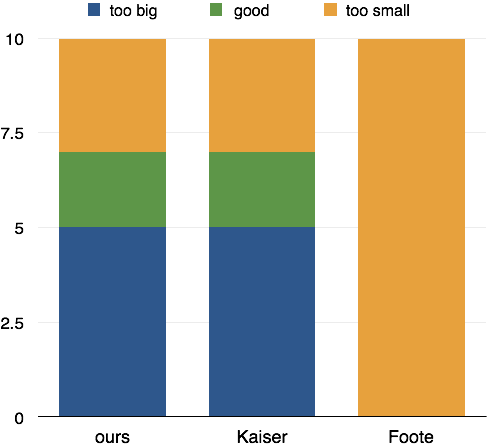
\includegraphics[width=0.48\textwidth]{Figures/count}
  \end{center}
  \caption{Figure presenting the amount of each type of errors produced by all the evaluated algorithms.}
\label{fig:boundcount}
\end{wrapfigure}

Another measurement of success of our boundary retrieval is computation of boundary detection hit-rate. A hit is counted whenever a reference boundary is within a certain window of an estimated boundary. An important thing to note is that each boundary should be matched at most once, otherwise we can get some irrelevant results. For instance, if we are estimating the algorithm with window size 3 seconds, in the ground truth there are two boundaries 6 seconds apart and our algorithm detects only one right in the middle, if we do not exclude the boundary once compared with the first one in the ground truth, the performance of our algorithm will be ranked as much better than it actually was. 


In addition to computing the hit-rate for windows of sizes 500ms and 3s, we also computed the median deviations between the reference and estimated boundaries of the song. In particular, we focused on median time from each reference boundary to the closest estimated boundary.

We implemented our evaluation benchmark using Python mir\textunderscore eval library \cite{mireval}.
Again, to best evaluate performance of our algorithm, we compare the results it yields with results of the checkerboard and NFM based ones. Our findings can be seen in Table \ref{table:evalStructureRank}.


\begin{wrapfigure}{r}{0.5\textwidth}
\vspace{-30pt}
  \begin{center}
    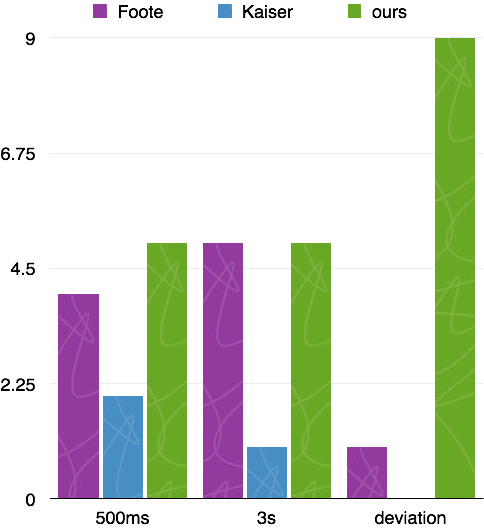
\includegraphics[width=0.48\textwidth]{Figures/structurechamps}
  \end{center}
  \caption{Chart presenting amount of times every algorithm excelled in each of the categories - hit-rate with window sizes of 500ms and 3s and the median deviation from the ground truth.}
\label{fig:structurechamps}
\end{wrapfigure}

As we can see in the Figure \ref{fig:structurechamps}, in the majority of cases, the performance of the algorithm designed by Kaiser falls behind the other two methods. It ranked as first twice when calculating the hit-rate with the window size w=500ms, once for the w=3s and it never excelled in the deviation category. On the other hand, the algorithm designed by Foote and Cooper yields similar overall performance as ours when evaluating hit-rate with w=3 and slightly worse for 500ms. This most probably is caused by the fact that in many cases our algorithm managed to find the segments but was a bit off, not qualifying for the 500s window. However, once the window got increased, its performance improved more than in case of the ``checkerboard'' algorithm. The exact results can be seen in section \ref{sec:segevalapp} in Appendix C. 

In conclusion, we believe that the algorithm for boundary detection we created is suitable for our application and yields performance comparable or exceeding the state-of-the-art creations in its field. 

\section{Labelling}


\section{Questionnaires}
Questionnaires are one of the most common and popular tools to gather data from a large number of people. They generally consist of a limited number of questions that ask participants to rate the effectiveness of various aspects of the activity. The questions should focus on the key points we are trying to evaluate. 

Questionnaires tend to be short in order to reduce the amount of time respondents need to complete them, and therefore increase the response rate. 

We composed questionnaires that are quantitative and generally consist of close-ended questions (tick the box, or scales), as the open ended questions tent to make data analysis and reporting more difficult.

\subsection*{Preliminary Research}

Before the design and implementation phase of the project, we conducted a study to determine what features could be desirable in the game. We led a survey among 18 people aged 17-25 asking about their past experience with music rhythm games. 
The questions and the results are presented in the Table \ref{table:preliminaryquestions}. Each of the questions was answered on a scale from 1 to 5, where 1 is a No,  3 is Neutral and 5 is a Yes.

\begin{table}
\begin{center}
\begin{tabular}{| p{8cm} | c | c | c | c | } 																								      \hline 
\textbf{Question} & \textbf{Average} & \textbf{Stdev} & \textbf{Min} & \textbf{Max} 						   \\ \hline \hline
Do you like playing games? & 4.11 & 0.9 & 2 & 5		 					 					 									\\ \hline 
Do you like listening to music? & 4.67 & 0.59 & 3 & 5		 					 					 								\\ \hline 
Do you often play games? & 3.722 & 0.89 & 2 & 5 		 					 					 								\\ \hline 
Have you ever played Guitar Hero or other rhythm music game? & 3.88 & 1.84  & 1 & 5							\\ \hline 
Did you feel like the choice of songs was limiting you? & 3.22 & 1 & 1 & 5 					 							\\ \hline 
Were you able to load in your song of choice in there? & 2. & 1.41 & 1 & 5 					 							\\ \hline 
Would you like to be able to load a song into it? & 4.27 & 0.82 & 3 & 5 				 									\\ \hline 
Did you feel like the game graphics were reflecting the emotions in the song? & 2.78 & 1.06 & 1 & 4 			\\ \hline 
Would you like the game to reflect the emotions in the song? & 3.67 & 0.84 & 3 & 5 	 								\\ \hline 
Was the game reflecting the section of the song you were in? & 2.44 & 1.25 & 1 & 4  								\\ \hline 
Do you feel it would be useful to know what section of the song is currently played? & 3.5 & 0.86 & 2 & 5  	\\ \hline 
\end{tabular}
\caption{Table presenting the results of the preliminary questionnaire.}
\label{table:preliminaryquestions}
\end{center}
\end{table}

As we can see from the Table \ref{table:preliminaryquestions}, the majority of young people surveyed did enjoy playing games to a similar extent. However, the results of the survey tell us that listening to music is almost unanimously beloved activity, with the highest average result and the smallest standard deviation. 
Majority of people play games quite often, but the lower average and standard deviation compared to the first question suggests that there are some people who enjoy playing games a lot but they do not spend that much time doing so, be it due to lack of time or other arrangements. 

When it comes to rhythm-games specific questions, most people have played a game of such type before. A majority of people believed that having a set playlist was limiting their experience, however, there were some who did not mind this that much. However, when asked if the ability to upload their own music would improve their experience, everybody was either neutral of agreed - nobody was against the idea. 

Majority, but no all surveyed believed that the rhythm game they played did not reflect the mood of the song they played, which can be deducted from the average below the neutral value 3 with the maximum value being four, so above the neutral. They believed it would be nice for the game to reflect the emotions in the song, but the need expressed was not as urgent as in case of the upload of their own songs. On the other hand, nobody opposed to such feature, which is reflected by the minimum value given being three.

Finally, we asked the surveyed whether they felt like the game was reflecting the built of the song, notifying them of where in the song they were. Most agreed that the games like that did not contain any sort of visualisation for the song segmentation. Majority of surveyed agreed that such feature would be useful, although a small amount of people believed it would not contribute in any way, answering with 2.

We also had to additional questions asking for suggestions, in case there are other features that could be useful to the game or could make the game more attractive that we missed in our initial market research. 

\subsection*{Final Research}

For our final research, we demonstrated our game to a group of 8 people aged 18-23 and asked them to fill in a questionnaire to describe their experience and thoughts on the game. Each of the questions was answered on a scale from 1 to 5, where 1 is a No,  3 is Neutral and 5 is a Yes. The questions and the results are presented in the Tables \ref{table:finalquestionsinterface}, .

\begin{table}
\begin{center}
\begin{tabular}{| p{8cm} | c | c | c | c | } 																	  \hline 
 \textbf{Question} & \textbf{Average} & \textbf{Stdev} & \textbf{Min} & \textbf{Max } \\ \hline \hline
 I knew what to do in the game straight away. 				& 4.88 & 0.35 & 4 & 5		   \\ \hline 
 I needed hints to play the game. 								& 2.25 & 1.58 & 1 & 5 	   \\ \hline 
 I needed somebody to tell me how to play the game. 	& 1.13 & 0.35 & 1 & 2  	   \\ \hline 
 I liked the design of the menu. 									& 3.86 & 0.99 & 2 & 5   	   \\ \hline 
 I felt like the game interface was too crowded. 				& 1.38 & 0.51 & 1 & 2 	   \\ \hline 
 I felt like the interface of the menu was too empty.		& 1.75 & 0.89 & 1 & 3		   \\ \hline
 I felt like i knew what each part was supposed to do. 	& 4.75 & 0.46 & 4 & 5		   \\ \hline
\end{tabular}
\caption{Table presenting the results of the final questionnaire concerning the game interface.}
\label{table:finalquestionsinterface}
\end{center}
\end{table}

As we can see, a vast majority found the user interface fairly straightforward. The rest of the interviewed needed hints provided in the game to fully understand the game play and the flow of the use. Almost nobody felt like they needed someone to explain what they are supposed to do in the game. 

More than half of the people liked the design of the menu - almost nobody felt like it was too crowded or too empty. In addition to this, the vast majority of the surveyed believed they could guess the purpose of the elements visible in the interface, with minimum response being 4.

\begin{table}
\begin{center}
\begin{tabular}{| p{8cm} | c | c | c | c | } 																			   \hline 
 \textbf{Question} & \textbf{Average} & \textbf{Stdev} & \textbf{Min} & \textbf{Max }	\\ \hline \hline
 The game was too difficult. 														& 2.86 & 0.83 & 2 & 4 \\ \hline		
 The game was too easy. 															& 1.13 & 0.35 & 1 & 2  \\ \hline
 The buttons felt synchronised with the game. 								& 3.75 & 0.46 & 3 & 4	 \\ \hline
 I noticed the changes in the mood influenced the game interface.	& 3.25 & 1.04 & 1 & 4	 \\ \hline
 I found the structure recognition useful.										& 4.00 & 0.35 & 3 & 5  \\ \hline
 I knew how to quit / pause / resume the game straight away.			& 4.88 & 0.83 & 4 & 5	 \\ \hline
 I knew how I was scored straight away.										& 4.13 & 0.93 & 3 & 5	 \\ \hline
 \end{tabular}
\caption{Table presenting the results of the final questionnaire concerning the gameplay.}
\label{table:finalquestionsgameplay}
\end{center}
\end{table}

The second set of questions was designed to find out about users' thoughts on the game itself. In the survey, we asked what the interviewees thought about the game's difficulty. The results can be seen in Table \ref{table:finalquestionsgameplay}. Nobody believed the game was too easy, with an average answer of 1.13 and maximum one being 2. The majority of the surveyed also thought that the game was not too difficult, although the average response was much closer to neutral. We believe that this is a desirable outcome, as the game is supposed to pose a challenge to the player or they will quickly become bored with it. 

We also focused on the assessment of individual elements that create the game experience and make it stand out from all the publications available on the market. The incorporation of the predominant melody detection as well as the button generation algorithm were referred to in a question about synchronisation between the music and the notes that come up on the screen. Every person asked either agreed or was neutral in response to the question. We believe the variation in the answers is due to different choice of songs the surveyed decided to upload. If the song did not have a one definite predominant melody from a single source, the buttons would become less predictable. 
We are satisfied with this score as the fact that nobody gave it less than 3 implies that the algorithms fulfill their purpose and generate relevant outputs in general.

The next question regarded the mood detection. Although the average response suggests that the users did notice the changes in the visuals triggered by the mood changes in the music, in fact, many people felt indifferent about this feature. When asked what they thought the reason was, they stated they were too focused on trying to ace the buttons to pay attention to the animation in the background.

We also asked about users' opinion on the structure retrieval system and its incorporation. Most people found it useful, claiming it helped them track where in the song they were. We believe the feature was a success as the lowest score it received was a neutral one. 

When asked about the controls, the all the users agreed that they were easy to find and use. In addition to this, they all felt that they new how the scoring worked and what to do to improve their results. 

\begin{table}
\begin{center}
\begin{tabular}{| p{8cm} | c | c | c | c | } 																			   \hline 
 \textbf{Question} & \textbf{Average} & \textbf{Stdev} & \textbf{Min} & \textbf{Max }	\\ \hline \hline
 I think the application does not require previous computer experience to be used properly. & 4.63 & 0.52 & 4 & 5 \\ \hline
 The buttons were designed in such way that the user can quickly become familiar with the game environment. & 4.38 & 0.52 & 4 & 5 \\ \hline
 The screens are well structured and their design is clear, aesthetic and attractive.  & 4.00 & 0.76 & 3 & 5 \\ \hline
 The amount of on-screen texts is not excessive. 	& 5.00 & 0.00 & 5 & 5 \\ \hline
 The fonts are clear and readable. 						& 3.38 & 0.74 & 3 & 5 \\ \hline
 The combination of colours is pleasing. 				& 4.38 & 0.74 & 3 & 5 \\ \hline
 \end{tabular}
\caption{Table presenting the results of the final questionnaire concerning the overall experience when playing the game.}
\label{table:finalquestionsoverall}
\end{center}
\end{table}

The final set of questions given to the surveyed asked them about their overall experience and thoughts on the application. Every person questioned believed to some extent that the application we created does not require the users to have previous computer experience to play - there was no answer below 4. This is really important, especially for a game, which we believe should be available and easy to use to everyone who wants to play it. 

The surveyed also appreciated the design of the buttons claiming their design helped to understand the flow of use.
They also believed that the structure of the screens was logical and visually pleasing. In addition to this, everybody unanimously agreed that the amount of the on-screen text was not excessive. This is encouraging, as very often games repel people by forcing them to read long lines of text. The colour scheme also received a favourable review, scoring an average of 4.38.

Most people believed that the fonts were clear and readable, but a few believed that a small increase in the font size would improve the user experience. 


 
%\input{Chapters/Chapter5} 
%\input{Chapters/Chapter6} 
%\input{Chapters/Chapter7} 

%----------------------------------------------------------------------------------------
%	BIBLIOGRAPHY
%----------------------------------------------------------------------------------------

\lhead{\emph{Bibliography}} % Change the page header to say "Bibliography"

\bibliographystyle{unsrtnat} % Use the "unsrtnat" BibTeX style for formatting the Bibliography
\bibliography{Bibliography} % The references (bibliography) information are stored in the file named "Bibliography.bib"


\end{document}  